\documentclass[conference]{IEEEtran}
\IEEEoverridecommandlockouts
% The preceding line is only needed to identify funding in the first footnote. If that is unneeded, please comment it out.
\usepackage{cite}
\usepackage{amsmath,amssymb,amsfonts}
\usepackage{graphicx}
\usepackage{textcomp}
\usepackage{xcolor}
\usepackage{titlesec}

\usepackage{textcomp}
\usepackage{epsfig}
\usepackage{algpseudocode}
\usepackage{pgfplots}
\usepackage{tikz}
\pgfplotsset{width=10cm,compat=1.9}
 \usepgfplotslibrary{external}
\usepackage{amsmath}
\usepackage{mathtools}
\DeclarePairedDelimiter{\floor}{\lfloor}{\rfloor}
\usepackage[linesnumbered,ruled,vlined]{algorithm2e}
\def\BibTeX{{\rm B\kern-.05em{\sc i\kern-.025em b}\kern-.08em
    T\kern-.1667em\lower.7ex\hbox{E}\kern-.125emX}}

\usepackage[ruled,vlined]{algorithm2e}

\tikzexternalize 
\begin{document}

\title{Finding shortest paths from source to all vertices in the given graph.\\
\text{\Large{DAA ASSIGNMENT-1 , GROUP 2}}
}
\author{\IEEEauthorblockN{Saloni Singla}
\IEEEauthorblockA{ \text{IIB2019004}}
\and
\IEEEauthorblockN{Sandeep kumar}
\IEEEauthorblockA{ \text{IIB2019005}}
\and
\IEEEauthorblockN{Amanjeet kumar}
\IEEEauthorblockA{ \text{IIB2019006}}
}

\maketitle

\begin{abstract}
This Paper contains the algorithm for finding shortest paths from source to all vertices in the given graph.
\end{abstract}

\section{Problem Statement}
Given a graph G and a starting source vertex s, what is the shortest paths from s to every other vertices of G.
\section{Keywords}
Graph, Dijkstra, Bellman-ford, Breadth-first-search

\section{Introduction}
The Single-Source Shortest Path (SSSP) problem consists of finding the shortest paths between a given vertex v and all other vertices in the graph.
\section{Algorithmic Design}

\subsection{ \textbf{Approach 1(By BFS on unweighted graph)}}
Breadth-first search (BFS) visits the nodes of a graph in increasing order of their distance from the starting node. Thus, we can calculate the distance from the starting node to all other nodes using breadth-first search.\\
Breadth-first search goes through the nodes one level after another. First the search explores the nodes whose distance from the starting node is 1, then the nodes whose distance is 2, and so on. This process continues until all nodes have been visited.

\begin{enumerate}
\item  The idea is to use a modified version of Breadth-first search in which we keep storing the predecessor of a given vertex while doing the breadth-first search. 
\item This algorithm will work even when negative weight cycles are present in the graph. 
\item We first initialize an array dist[0, 1, …., v-1]  such that dist[i] stores the distance of vertex i from the source vertex.
\item Now we get the length of the path from source to any other vertex in O(1) time from array d, and for printing the path from source to any vertex we can use array p and that will take O(V) time in worst case as V is the size of array P. 
\item So most of the time of the algorithm is spent in doing the Breadth-first search from a given source which we know takes O(V+E) time. Thus the time complexity of our algorithm is O(V+E). 
\end{enumerate}

\subsection{ \textbf{Approach 2(By Dijkstra on weighted Graph(with Positive weights)}}
Dijkstra's algorithm can be used for non-negative weight edges, Dijkstra's algorithm has many variants but the most common one is to find the shortest paths from the source vertex to all other vertices in the graph.

\begin{enumerate}
\item Dijkstra’s  algorithm set all vertices distances to infinity except for the source vertex and it sets the source distance to 0. 
\item Dijkstra’s  algorithm  is  efficient of all algorithms,because it  only  processes  each  edge  in  the  graph only once by assuming  that there are no negative edges.
\item Dijkstra’s algorithm calculates the distances from the node to other nodes of the graph and stores in a mi-priority queue to compare in the form of (distance , vertex). The nodes are ordered   by  their  distances. 
\item Using  a priority queue, the next node to be processed can be retrieved in logarithmic time. The queue gets updated to the distance from the current vertex + edge weight. And if the popped vertex is visited before it continues without using it. It is Applied again until the priority queue is empty.
\end{enumerate}

\subsection{ \textbf{Approach 3(By Bellman-Ford on weighted Graph(with negative weights))}}
The Bellman–Ford algorithm finds shortest paths from a starting node to all nodes of the graph. The algorithm can process all kinds of graphs, provided that the graph does not contain a cycle with negative length. If the graph contains a negative cycle, the algorithm can detect this.\\ 
The algorithm keeps track of distances from the starting node to all nodes of the graph. Initially, the distance to the starting node is 0 and the distance to any other node is infinite. The algorithm then reduces the distances by finding edges that shorten the paths until it is not possible to reduce any distance.

\begin{enumerate}
\item The main idea of this algorithm is simple: Relax all E edges (in arbitrary order) V -1 times!
\item Initially dist[s] = 0, the base case. If we relax an edge s → u, then dist[u] will have the correct value.
\item If we then relax an edge u → v, then dist[v] will also have the correct value. 
\item If we have relaxed all E edges V -1 times, then the shortest path from the source vertex to the furthest vertex from the source (which will be a simple path with V -1 edges) should have been correctly computed.

\end{enumerate}

\end{enumerate}

\newline
\begin{algorithm}
    \caption{To find SSSP in an unweighted graph using BFS.}
    \KwIn{source src,adjacency list l}
    \KwOut {distance array}
    \DontPrintSemicolon
     \SetKwFunction{FMain}{BFS}
    \SetKwProg{Fn}{Function}{:}{}
    \Fn{\FMain{$src,l$}}{ 

        $dist[src]\gets INT\_MAX$\;
        $distance[src]\gets0$\;
        $q.push(src)$\;
        \While{$q.empty()=false$}{
            $parent\gets q.front()$\;
            $q.pop()$\;
            \For{$auto$\text{ }$nbr$\text{ : }$l[parent]$ }{
                \If{$dist[nbr]=INT\_MAX$}{
                    $q.push(nbr)$\;
                   $distance[nbr]\gets distance[parent]+1$\;
                }
            }
        }
    }
\end{algorithm}

\begin{algorithm}


   \caption{Dijkstra's Algorithm}
    \KwIn{source $s$,no. of vertex $n$,adjacency list $vec$}
    \KwOut{$dist$ array}
    \SetKwInOut{KwRequire}{Require}
    % \KwRequire{$n\geq 0$}
    \DontPrintSemicolon
    \SetKwFunction{FMain}{SSSP}
    \SetKwProg{Fn}{Function}{:}{}
    \Fn{\FMain{$src,n,vec$}}{ 
       \For{$i\gets 0$ \text{ to } $n-1$}{
        $dist[i]\gets Inf$\;
       }
       $dist[s]\gets0$\;
       \For{$i\gets 0$ \text{ to } $n-1$}{
        $visited[i]\gets false$\;
       }
       $visited[s]\gets true$\;
       $p.push({0,s})$\;
       \While{$q.empty()=false$}{
        $t\gets p.top()$\;
        $p.pop()$\;
        $visited[t.second]\gets true$\;
         \For{$i\gets0 $ \text{ to } $vec[t.second].size()-1$}{
        $visited[i]\gets false$\;
        \If{$ visited[vec[t.second][i].first] = false$ $AND$ $ t.first+vec[t.second][i].second<distance[vec[t.second][i].first]$}{
            $distance[vec[t.second][i].first]\gets t.first+vec[t.second][i].second$\;
            $p.push({distance[vec[t.second][i].first],vec[t.second][i].first})$\;
            
        }
       }
       }
    }
    
\end{algorithm}

\begin{algorithm}

    \caption{Bellman's Algorithm}
    \KwIn{source $s$, no. of nodes $V$,adjacency list $AdjList$}
    \KwOut{$dist$ array}
    \SetKwInOut{KwRequire}{Require}
    % \KwRequire{$n\geq 0$}
    \DontPrintSemicolon
    \SetKwFunction{FMain}{SSSP}
    \SetKwProg{Fn}{Function}{:}{}

    \Fn{\FMain{$s,V,AdjList$}}{ 
       \For{$i\gets 0$ \text{ to } $V-1$}{
        $dist[i]\gets Inf$\;
       }
       $dist[s]\gets0$\;
        \For{$i\gets 0$ \text{ to } $V-2$ }{
                \For{$u\gets 0$ \text{ to } $V-1$ }{
                    \For{$j\gets 0$ \text{ to } $(int)AdjList[u].size()$ }{
                    $v\gets AdjList[u][j]$\;
                    $dist[v.first]\gets min(dist[v.first], dist[u] + v.second)$\;
                }
            }
       }
    }
    
\end{algorithm}

\newpage
% Continue.....

\section{Algorithm Analysis}

\subsection{\textbf{TimeComplexity}}
Approach  1: Time  complexity  of  breadth  first  search(BFS) is O(V+E),  where V is  the  number  of  nodes  and E is  the number of edges.\\
Approach  2: Time  complexity  of  Dijkstra’s  algorithm  is O($V+E logE$), because it goes through all nodes of  the  graph  and adds the distance for maximum of one time when at the current node.\\
Approach  3: Time  complexity  of  Bellman Ford's algorithm  is O($V*E$),  because  it consists  of ($V−1$) rounds  and iterates through all E edges during a round.

\subsection{\textbf{Space Complexity}} 
The  space  complexity  for  BFS and Dijkstra’s algorithms  is [$O(V+E)$ (for  adjacency  list)  + $O(V)$ (for  other  arrays)],  and  for Bellman Ford's  algorithm,  the complexity is O(V) +O(E).

\section{Experimental study}

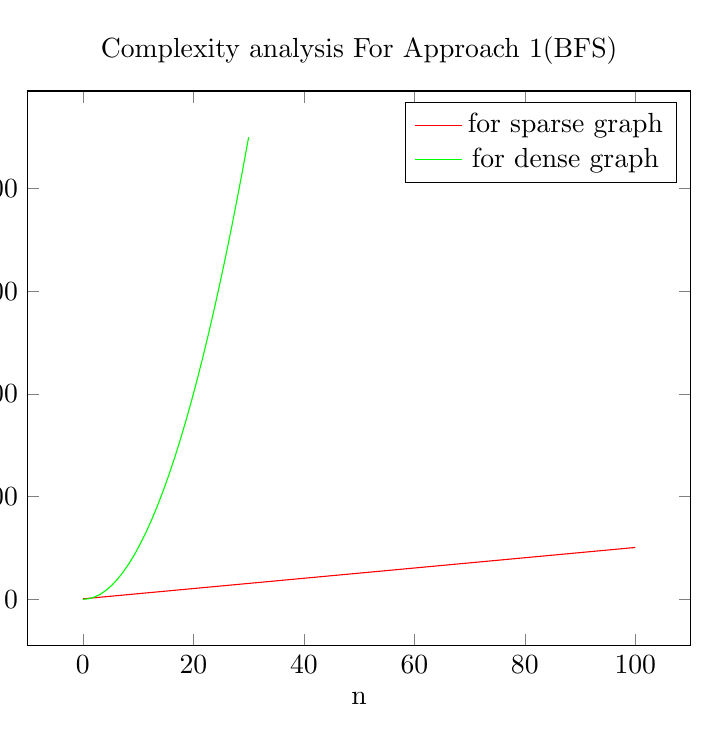
\begin{tikzpicture}[trim left=0cm]
\begin{axis}[
    title={Complexity analysis For Approach 1(BFS)},
    xlabel={n},
    ylabel={Time taken in (ms)},
]
    %Here the blue parabloa is defined
\addplot [
    domain=0:100,
    samples=1000, 
    color=red,
    ]
    {x+1};
\addlegendentry{for sparse graph}
%Below the red parabola is defined
\addplot [
    domain=0:30,
    samples=30,
    color=green,
]
{x^2};
\addlegendentry{for dense graph}
   \end{axis}
   
\end{tikzpicture}


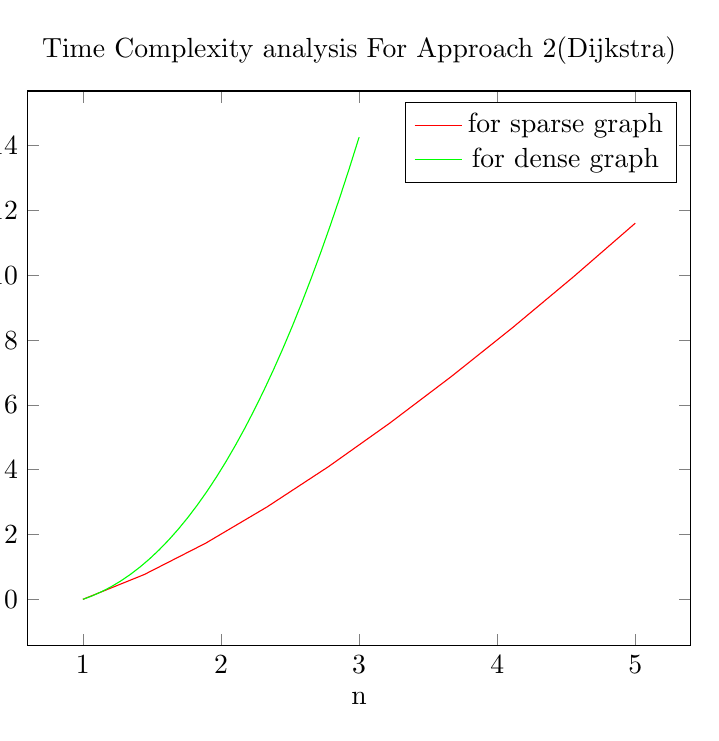
\begin{tikzpicture}[trim left=0cm]
\begin{axis}[
    title={Time Complexity analysis For Approach 2(Dijkstra)},
    xlabel={n},
    ylabel={Time taken in(ms)},
]

\addplot [
    domain=1:5, 
    samples=10, 
    color=red,
    ]
    {x*log2(x)};
\addlegendentry{for sparse graph}

\addplot [
    domain=1:3, 
    samples=30, 
    color=green,
]
{(x^2)*log2(x)};
\addlegendentry{for dense graph}
\end{axis}
\end{tikzpicture}



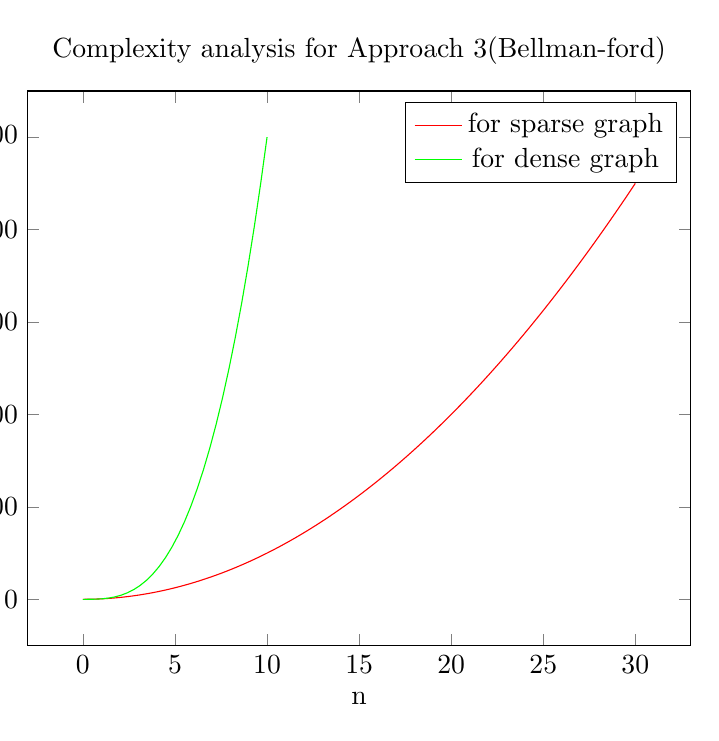
\begin{tikzpicture}[trim left=0cm]
\begin{axis}[
    title={Complexity analysis for Approach 3(Bellman-ford)},
    xlabel={n},
    ylabel={Time taken in(ms)},
]
%Here the blue parabloa is defined
\addplot [
    domain=0:30, 
    samples=100, 
    color=red,
    ]
    {x^2};
\addlegendentry{for sparse graph}
%Below the red parabola is defined
\addplot [
    domain=0:10, 
    samples=30, 
    color=green,
]
{(x^3)};
\addlegendentry{for dense graph}
  \end{axis}
  \end{tikzpicture}
  
\section{Conclusion}
Here we discussed algorithms to solve SSSP for undirected graph and also  for Unweighted graph, the distances can be computed in almost linear time complexity but for weighted graph, there exist several algorithms for different types of graphs.
\section{REFERENCES}
    \item \url{https://www.geeksforgeeks.org/dijkstras-shortest-path-algorithm-greedy-algo-7/}
    \item \url{https://www.geeksforgeeks.org/shortest-path-unweighted-graph/}
    \item \url{https://www.geeksforgeeks.org/bellman-ford-algorithm-dp-23/}
    


\end{document}
